\ylDisplay{Läätsed} % Ülesande nimi
{Tundmatu autor} % Autor
{lõppvoor} % Voor
{2014} % Aasta
{P 3} % Ülesande nr.
{2} % Raskustase
{
% Teema: Valgusõpetus
\ifStatement
Optiline süsteem koosneb kumerläätsest fookuskaugusega $f_1$ ning nõgusläätsest fookuskaugusega $f_2$, kusjuures $f_1 = -4f_2$. Läätsed on paigutatud nii, et nende optilised peateljed ühtivad ning nende vaheline kaugus on $1,5f_1$. Ese asub kumerläätsest kaugusel $2f_1$. Konstrueerige eseme kujutis optilises süsteemis. 
\begin{center}
	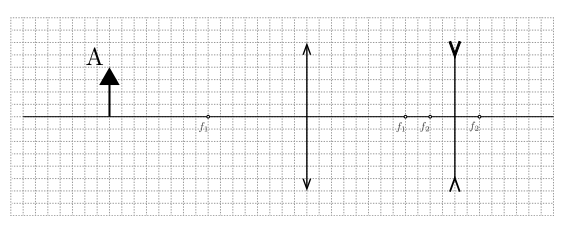
\includegraphics[width=0.5\linewidth]{2014-v3p-03-yl.PNG}
\end{center}
\fi
\ifHint
Konstrueerimisel peab järgima koondava kumerläätse ja hajutava nõgusläätse seaduspärasusi.
\fi
\ifSolution
\begin{center}
	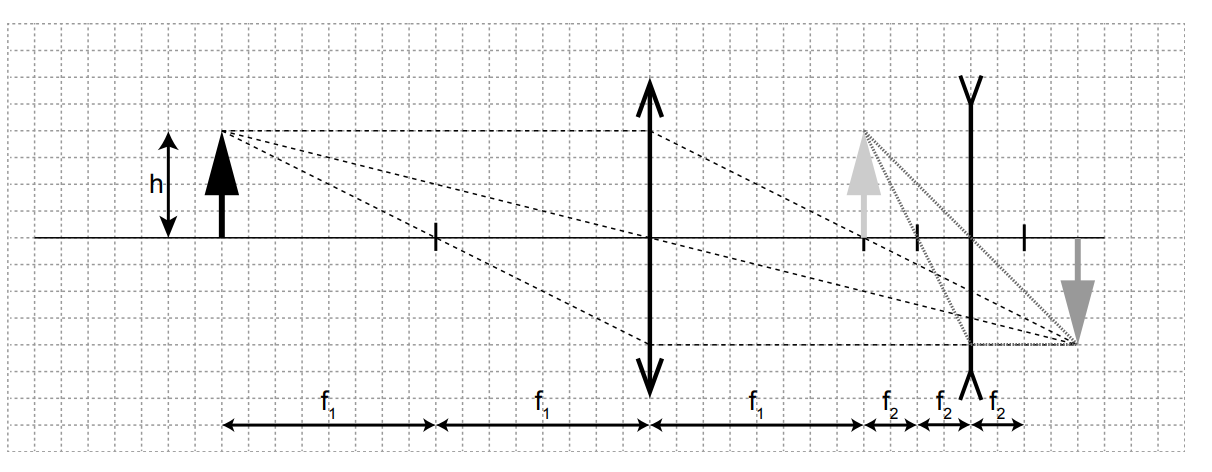
\includegraphics[width=0.5\linewidth]{2014-v3p-03-lah.PNG}
\end{center}
\fi
}
 
